\section{Discussions and Future Work}
\label{sec:discuss}
% Last paragraph of \S\ref{sec:accuracy:trace} discusses impact of task skew on
% \slearn's prediction accuracy and \S\ref{sec:back:jobmodel} discusses . Here 

%We discuss several design issues and extensions of \slearn.

\paragraph{Robustness to task skew.} There are two factors
that can potentially cause high variations in the runtime properties
of tasks (\textit{skew}) of a job: heterogeneity in cluster and
computation skew.
{
The three traces used in our analysis (\S\ref{sec:accuracy:trace}) and experiments
(\S\ref{sec:study}) are from production datacenter traces, out of
which, the Google traces were collected from 
heterogeneous clusters which already include task skew due to cluster
heterogeneity,
% Furthermore, our experimental analysis for prediction accuracy in
% \S\ref{sec:accuracy:experiment} and end-to-end performance analysis in
% \S\ref{sec:study} have shown better results for learning in space as
% compared to learning in time for the trace.
% Additionaly, previous work like LATE~\cite{late:osdi08} have established mechanisms to tame skew
%  in highly heterogeneous environments.
and all traces {already} include computation skew observed in 
real applications.
%
\if 0
We also expect the real workload in other production datacenters to have similar
task skew as previous work such as LATE~\cite{late:osdi08} has argued \comment{shown???}
why the tasks of the same job or of the same phase of a multi-phase
job will inherently be required to do roughly the same amount of work
and hence likely leads to low task skew.
\fi
Our analysis shows that for such real-world
traces, sampling-based learning outperforms the state-of-the-art
history-based learning scheme in terms of trace variability (\S\ref{sec:accuracy:trace}),
prediction accuracy (\S\ref{sec:accuracy:experiment}) as well as
end-to-end performance (\S\ref{sec:study:sim}).
%   Other work such as
%   SkewReduce~\cite{skewReduce:socc2010} developed mechanisms to tackle
%   inflation of computation skew.  }

\if 0
\input deadline-design
\fi

\paragraph{Combining history and sampling.}
There are several motivations for exploring combining history-
and sampling-based learning. 
%
(1) For mixed workloads, sampling-based learning can be used
to estimate the mean task length to minimize the total completion
time for jobs without deadlines, while history-based learning can be
used to estimate the max task length for deadline jobs, if it
can achieve comparable accuracy as 
sampling-based learning but without incurring any runtime overhead.
%   deadlines needs knowledge of both the average task
% length and the maximum task length. Our initial study has shown that,
% without any knowledge about the task length distribtuion, the
% prediction accuracy for max task length is about the same for both
% history and sampling-based schemes. However, since 
(2) History-based learning can be used to establish a prior
distribution, and sampling-based approach can be used to refine the
posterior distribution. Such a combination may potentially be more accurate
than using either history or sampling alone. For example,
knowing the distribution of task lengths can help develop better
max task length predictors.
(3) Finally, though not seen in the production traces used in our study,
in case task-wise variation and job-wise variation fluctuate, adaptively switching
between the two prediction schemes may help.


\questionaj{I am working on getting a figure here to show evidence for merging History and Sampling. The figure will have two curves. The values to plot will be calculated as similar to what is done for fig. \ref{fig:accuracy:trace_analysis_window}. There will be two curves, one will show CoV in average task duration for jobs corresponding to a feature\_value and another will show CoV in their CoVs.}

%
\begin{figure}[tp]
\centering
\vspace{-0.15in}
\subfigure[2STrace]
{
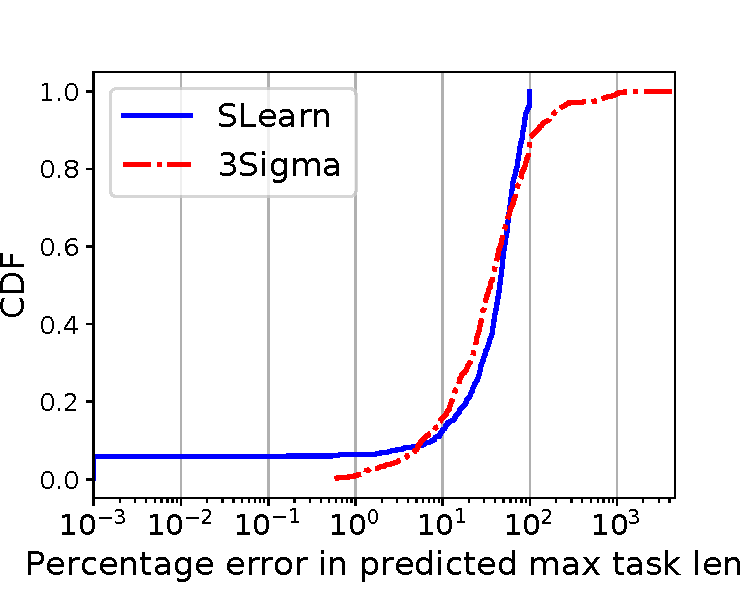
\includegraphics[width=0.49\linewidth]{figures/simulation/prediction_error_maxTask_new_2STrace.pdf}
\label{fig:sim:estimationAccuracy-max:2STrace}
}
\hspace{-0.15in}
\subfigure[GTrace]
{
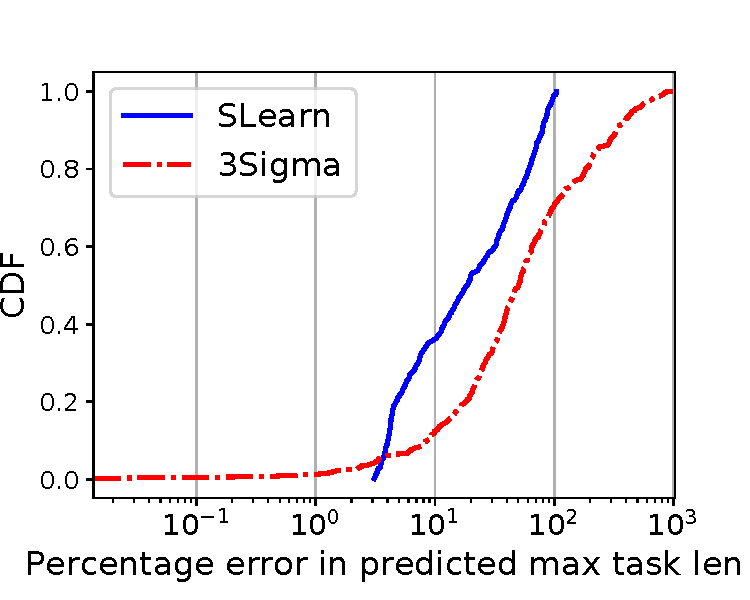
\includegraphics[width=0.49\linewidth]{figures/simulation/prediction_error_maxTask_new_gTrace.pdf}
\label{fig:sim:estimationAccuracy-max:GTrace}
}
\vspace{-0.15in}
\caption{Max runtime prediction accuracy.}
\vspace{-0.15in}
\label{fig:sim:estimationAccuracy-max}
\end{figure}
\begin{figure}[tp]
\centering
%\vspace{-0.15in}
	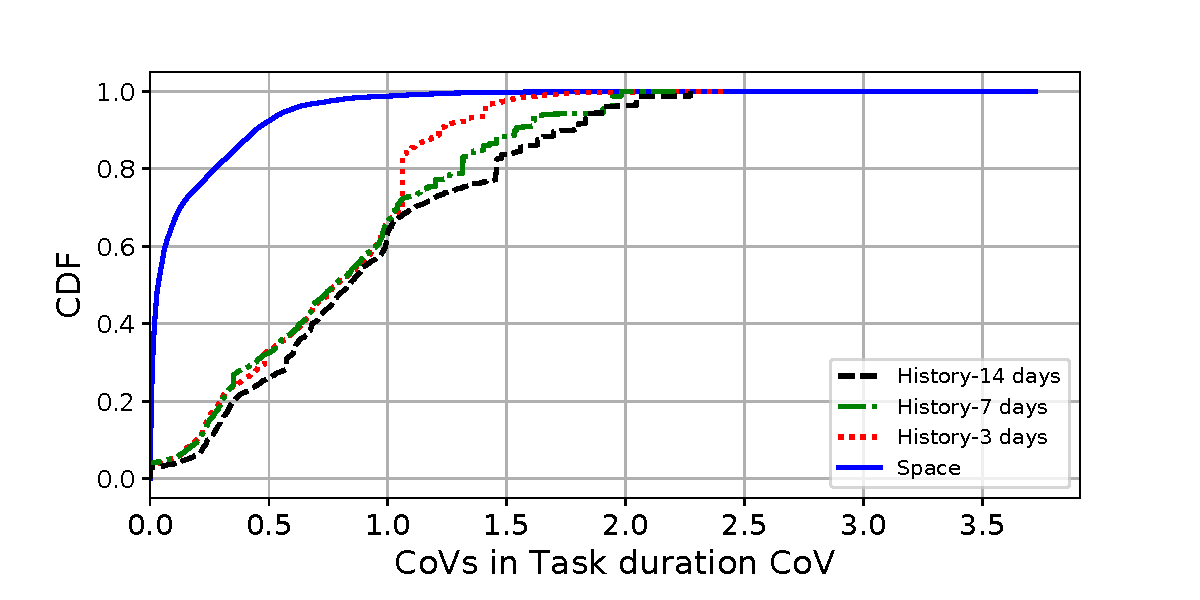
\includegraphics{figures/trace_analysis/slidingWindow_analysis_unified_cdf_of_covs_in_task_dur_cov_for_user_name_in_google11-with_space.pdf}
\caption{CoV of Task-Duration-CoV. The blue curve is CoV in task duration. This is for proof of concept of using history to predict CoV of task duration of job. So we can find an bound to error for the job.}
%\vspace{-0.15in}
\label{fig:sim:estimationAccuracy-max}
\end{figure}
\paragraph{Learning for whole DAG jobs.}
For multi-phase DAG jobs, the sampling-based prediction scheme can be
applied in each phase to optimize the performance (\eg completion
time) of each phase.  An interesting question is how to apply sampling
if we wish to learn the runtime 
properties of and optimize the performance of each multi-phase job {as a
  whole} (\eg~\cite{jockey:eurosys2012, AltruisticScheduling}).  We
expect that in that case it may again be helpful to combine
history-based prediction of the parameters of future phases with
sampling-based prediction of the current phase, which we plan to study
in future work.


%for jobs without deadlines (so that we can
%minimize their total completion time), while history-based learning can be
%used for jobs with deadline. As
%observed in \S\ref{sec:accuracy} and \S\ref{sec:study}, sampling works better
%than history for minimizing the completion time. However, for predicting
%Thus, history-based learning could be better for jobs with deadlines,
%since it takes zero runtime overhead.


\if 0
\paragraph{Dynamic adjustment of ThinLimit}
\questionaj{I have mentioned certain things in the \S\ref{sec:design:gs}. What
we discussed earlier to present that certain percentage of thin jobs should be
ideal seems not very true with the data. For the 2STrace with TL = 6 thin
jobs are 37\%. For the GTrace with TL = 3 (optimal configuration for the
GTrace.) thin jobs are 44\% and with TL = 6 thin jobs are 50\% (For the GTrace
these stats are after omitting single task jobs. We did so because the
fraction of single task jobs is very high.).}
\fi

